%% Digital Systems
%% Continuous System Equivalence
\def\FileDate{10/01/21}
\def\FileVersion{1.0}
% ----------------------------------------------------------------
% Notes pages *********************************************************
% ----------------------------------------------------------------

\begin{slide}
	\heading{Purpose of this Lecture}
	To describe the basic tools for the design of a control system to be implemented using a computer or microcomputer.

	\textbf{Contents}
	\begin{itemize}
		\item Typical architecture
		\item Relationship between $s$ and $z$
		\item Continuous design followed by digitisation
		\item Direct digital design
	\end{itemize}
\end{slide}

\section*{Typical Architecture of a Digital Control System}

\begin{slide}
	\heading{Typical Architecture}
	\begin{center}
	\resizebox{300pt}{!}{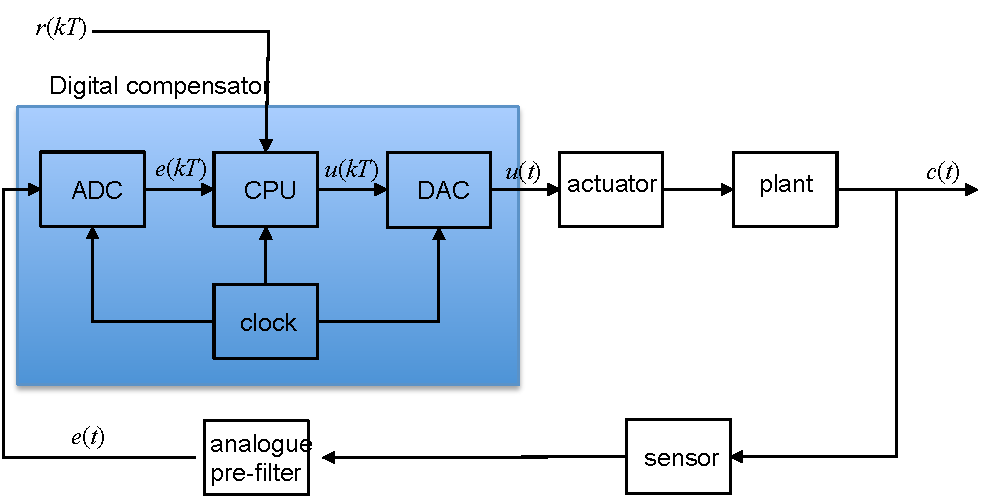
\includegraphics{pictures/digicon.pdf}}
\end{center}
\end{slide}

\section*{Relationship between $s$ and $z$}

We have already seen (SLIDE~2, lecture 11) that
\begin{equation}\label{eq:l12e1a}
	z=e^{sT}
\end{equation}
and
\begin{equation}\label{eq:l12e1b}
	s=\frac{1}{T}\ln z
\end{equation}
We can use Equation~\ref{eq:l12e1a} to define a mapping between the $s$ and $z$ planes as summarised in SLIDES~\ref{slide:l12s2} and \sref{slide:l12s3}.
\begin{slide}\label{slide:l12s2}
  \heading{Mapping between between $s$ and $z$}
  Since $z=e^{sT}$ we can define a `mapping' from the $s$-plane to the $z$-plane. Various properties of the $z$-plane follow.
\begin{itemize}
  \item s-plane stability boundary $s=j\omega$ maps to the unit circle $|z|=1$ in the z-plane.
  \item Maximum frequency is half the sampling frequency $\omega_s/2$ (a consequence of Nyquist's sampling theorem) and is mapped to the negative real axis in the z-plane.
\end{itemize}
For proofs, see the problems in the self-directed learning exercises.
\end{slide}

\begin{slide}\label{slide:l12s3}
  \heading{Stability in the z-plane}
\begin{itemize}
  \item Because the stability boundary is a unit circle, Routh-Hurwitz and Nyquist stability tests no longer work.
  \item The Jury test is a similar test to the Routh-Hurwitz test but it is more involved.
  \item The design curves for constant natural frequency $\omega_n$, damping ratio $\zeta$, $\sigma_d$ and $\omega_d$ are also distorted by the mapping.
  \item Use the Matlab function \emph{zgrid} to see the mapping.
\end{itemize}
\end{slide}

\begin{slide}\label{slide:l12s4}
  \heading{z-plane Design Curves}
  \begin{center}
    \scalebox{0.3}{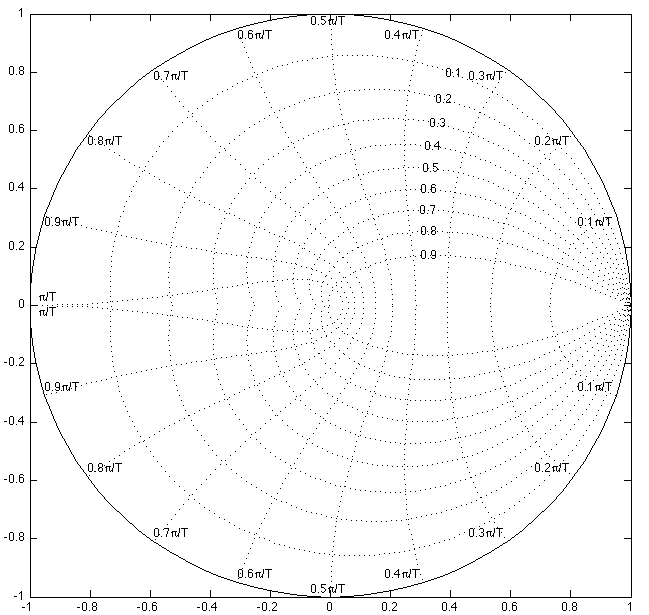
\includegraphics{pictures/zgrid.png}}
  \end{center}
\end{slide}


\section*{Continuous Design}

\begin{slide}
	\heading{Digitization Procedure}
	Given a continuous $D(s)$ find best equivalent $D(z)$.
	\begin{center}
		\resizebox{200pt}{!}{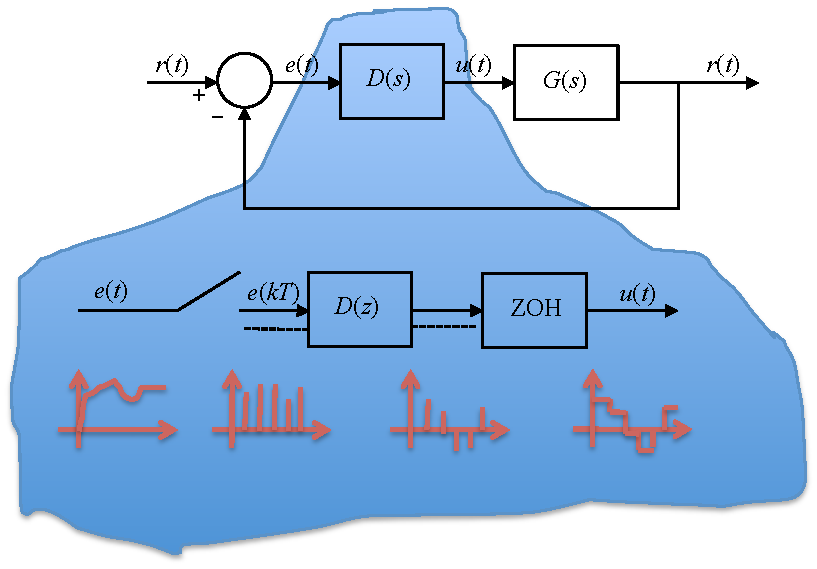
\includegraphics{pictures/digitization.pdf}}
	\end{center}
\end{slide}

There is no exact solution since the whole time history is available to $D(s)$ whereas only samples are available to $D(z)$ so different digitisation approximation methods make different assumptions about what happens to $e(t)$ between sampling instants.

\begin{slide}
	\heading{Summary of Digitization Methods}
	See Lecture 11 for mathematical derivations.
\end{slide}


\subsection*{Continuous Design}

\subsection*{Limits of Continuous Design Approach}

If an exact discrete analysis or a simulation of a system were performed and digitisation determined for a large range of sampling rates the digitised system would be unstable for rates slower than approximately $5\omega_n$ (where $\omega_n$ is the natural frequency of the system dominant poles) and damping would be degraded for rates slower than $10\omega_n$. At sampling rates higher than $20\omega_n$ (or $20\times \omega_{BW}$ for more complex systems) then all methods yield reasonable results and can be used with confidence at rates of $30\times \omega_{BW}$ or higher.

Errors come about because the approximations ignore the phase lag effect of the zero-order-hold (ZOH). The ZOH can be approximated by $$G_{zoh}(s)\approx \frac{2/T}{s+(2/T)}$$ which is based on the idea that, on average, the ZOH delays the signal by about $T/2$ seconds and this transfer function is a first-order lag with time constant $T/2$ and DC gain of 1. If this was added to the plant transfer function then a more accurate model of the delayed plant wiould be obtained and a more stable design for $D(s)$.

However, the advantage of continuous design is that $T$ is not chosen until after $D(s)$ is designed and the appearance of $T$ so early invalidates this assumption.

\section*{Direct Digital Design}

%----------------------------------------------------------------
% The end of notes
% ----------------------------------------------------------------
\endinput

% Local Variables:
% TeX-master: "lecture03"
% End:
